\documentclass{vgtc}                          % final (conference style)
%\documentclass[review]{vgtc}                 % review
%\documentclass[widereview]{vgtc}             % wide-spaced review
%\documentclass[preprint]{vgtc}               % preprint
%\documentclass[electronic]{vgtc}             % electronic version

%% Uncomment one of the lines above depending on where your paper is
%% in the conference process. ``review'' and ``widereview'' are for review
%% submission, ``preprint'' is for pre-publication, and the final version
%% doesn't use a specific qualifier. Further, ``electronic'' includes
%% hyperreferences for more convenient online viewing.

%% Please use one of the ``review'' options in combination with the
%% assigned online id (see below) ONLY if your paper uses a double blind
%% review process. Some conferences, like IEEE Vis and InfoVis, have NOT
%% in the past.

%% Figures should be in CMYK or Grey scale format, otherwise, colour 
%% shifting may occur during the printing process.

%% These three lines bring in essential packages: ``mathptmx'' for Type 1 
%% typefaces, ``graphicx'' for inclusion of EPS figures. and ``times''
%% for proper handling of the times font family.

\usepackage{mathptmx}
\usepackage{graphicx}
\usepackage{times}
\usepackage{subfigure}

%% We encourage the use of mathptmx for consistent usage of times font
%% throughout the proceedings. However, if you encounter conflicts
%% with other math-related packages, you may want to disable it.

%% If you are submitting a paper to a conference for review with a double
%% blind reviewing process, please replace the value ``0'' below with your
%% OnlineID. Otherwise, you may safely leave it at ``0''.
\onlineid{0}

%% declare the category of your paper, only shown in review mode
\vgtccategory{Research}

%% allow for this line if you want the electronic option to work properly
\vgtcinsertpkg

%% In preprint mode you may define your own headline.
%\preprinttext{To appear in an IEEE VGTC sponsored conference.}

%% Paper title.

\title{OpenSpace: Public Dissemination of Space Mission Profiles}

\author{Alexander~Bock\thanks{e-mail: alexander.bock@liu.se}\\%
        \scriptsize Link\"oping University
\and Michal Marcinkowski\thanks{e-mail:micma909@student.liu.se}\\ %
     \parbox{1in}{\scriptsize \centering American Museum of Natural History \\ Link\"oping University}
\and Joakim Kilby\thanks{e-mail:joakim.kilby@liu.se}\\ %
        \scriptsize Link\"oping University
\and Carter Emmart\thanks{e-mail:carter@amnh.org}\\%
        \parbox{1in}{\centering \scriptsize American Museum of Natural History}
\and Anders Ynnerman\thanks{e-mail:anders.ynnerman@liu.se}\\%
        \scriptsize Link\"oping University
}

% A teaser figure can be included as follows, but is not recommended since
%% the space is now taken up by a full width abstract.
\teaser{
\newcommand{\abTeaserHeight}{0.325\linewidth}
\subfigure[New Horizons space craft and Pluto] {
  \fbox{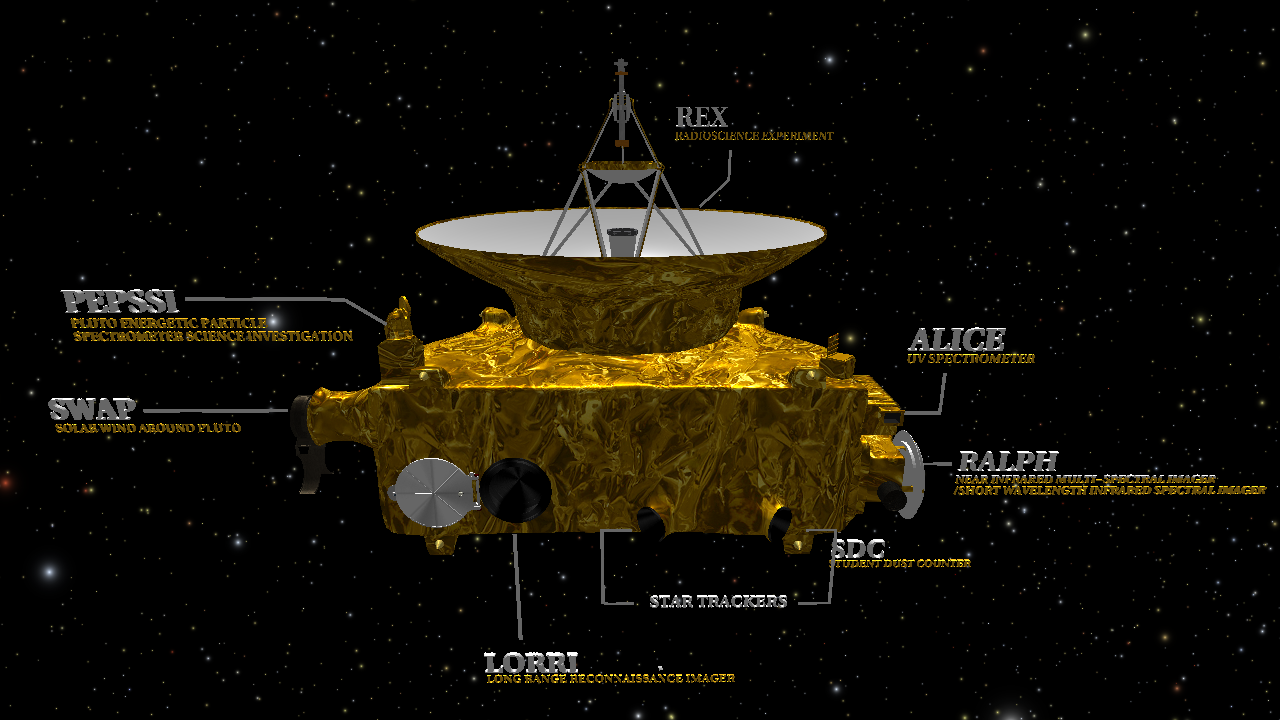
\includegraphics[height=\abTeaserHeight]{figures/newhorizons.png}}
  \label{fig:teaser:nh}
}
\subfigure[67P Churyumov-Gerasimenko] {
  \fbox{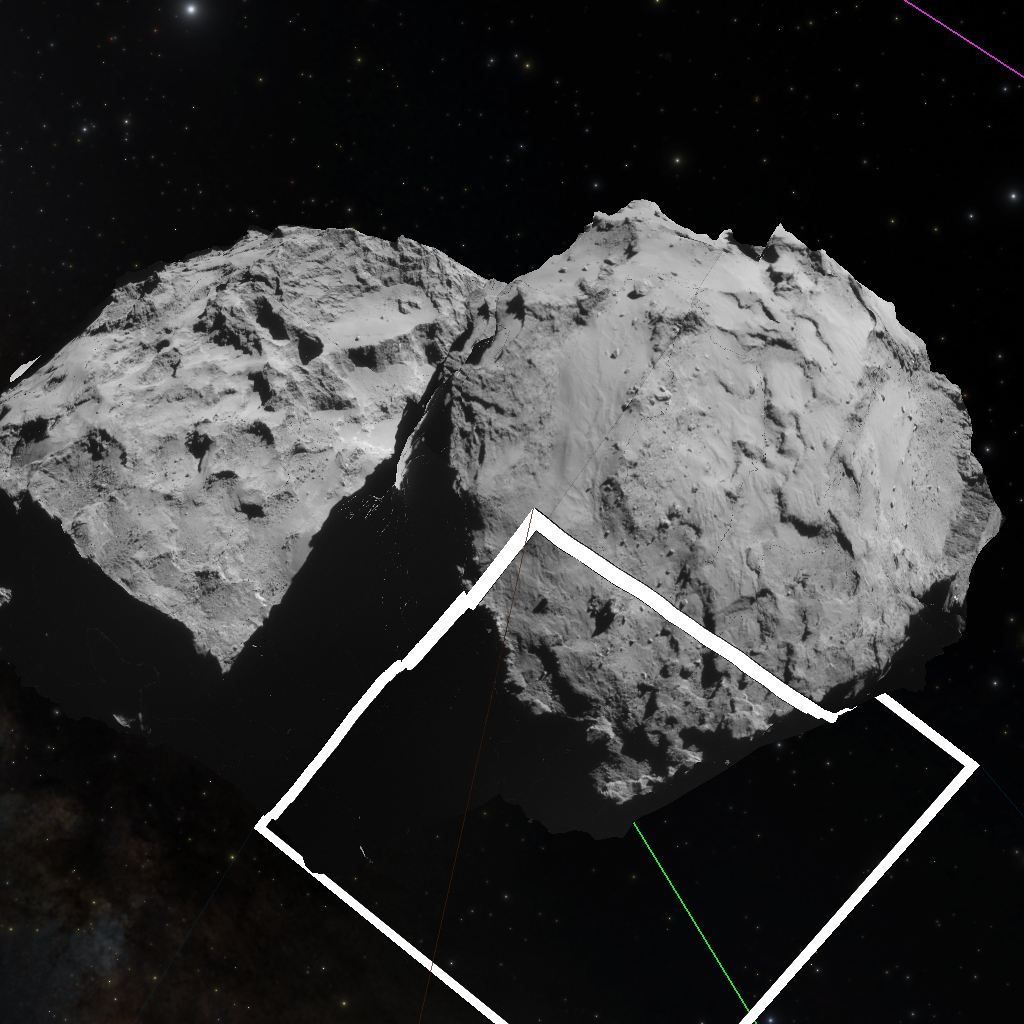
\includegraphics[height=\abTeaserHeight]{figures/67p.jpg}}
  \label{fig:teaser:67p}
}  
\caption{Examples of space mission visualization in our proposed system. (a) The New Horizons space craft with annotated science instruments in front of Pluto, providing the audience with the knowledge about the available instruments. (b) Images of the Rosetta orbiter's Navcam projected onto 67P, producing a high-fidelity rendering of the comet it orbits.}
\label{fig:teaser}
}

\abstract{This work presents a visualization system and its application to space missions. The system allows the public to disseminate the scientific findings of space craft and gain a greater understanding thereof. Instruments' field-of-views and their measurements are embedded in an accurate 3 dimensional rendering of the solar system to provide context to past measurements or the planning of future events. We tested our system with NASA's \emph{New Horizons} at the Pluto Pallooza event in New York and will expose it to the greater public on the upcoming July 14th Pluto flyby.}

\setlength\fboxsep{0pt}

\begin{document}
\firstsection{Introduction}
\maketitle

\begin{figure*}
\centering
\newcommand{\abOverviewWidth}{0.32\linewidth}
\subfigure[Image projection onto Jupiter] {
  \fbox{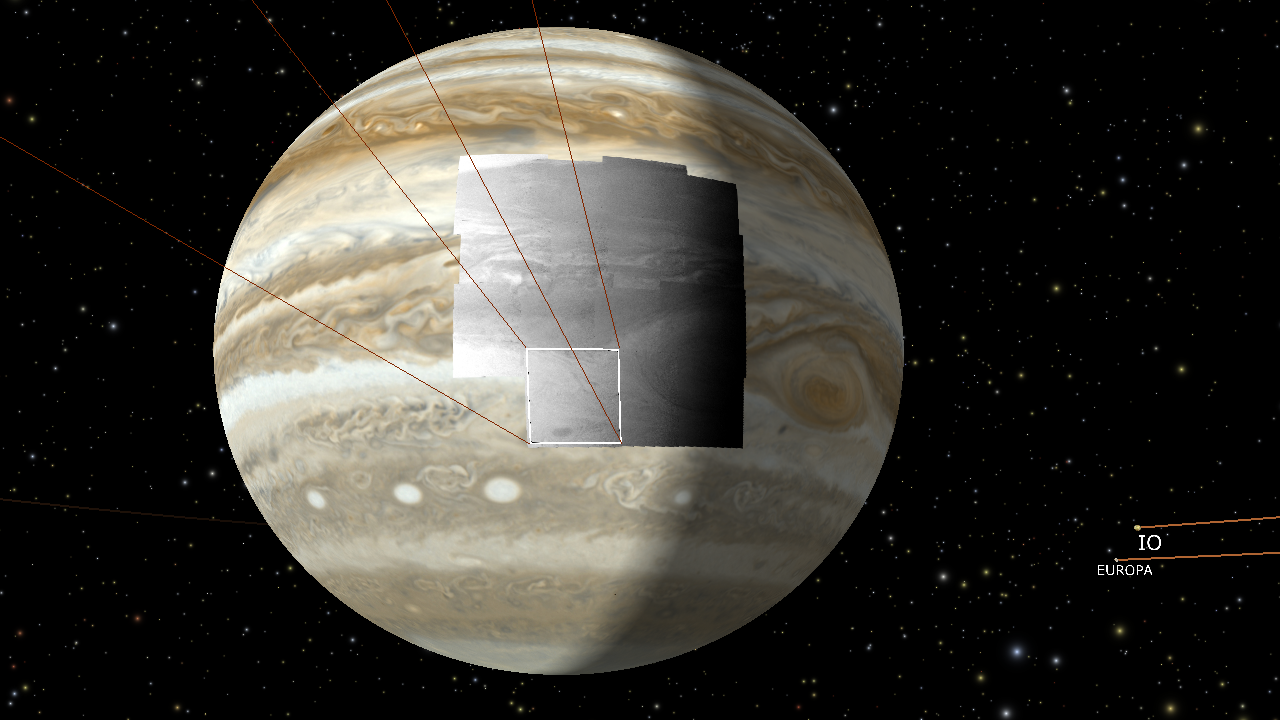
\includegraphics[width=\abOverviewWidth]{figures/jupiter.png}}
  \label{fig:jupiter}
}
\subfigure[Image projection onto Pluto] {
  \fbox{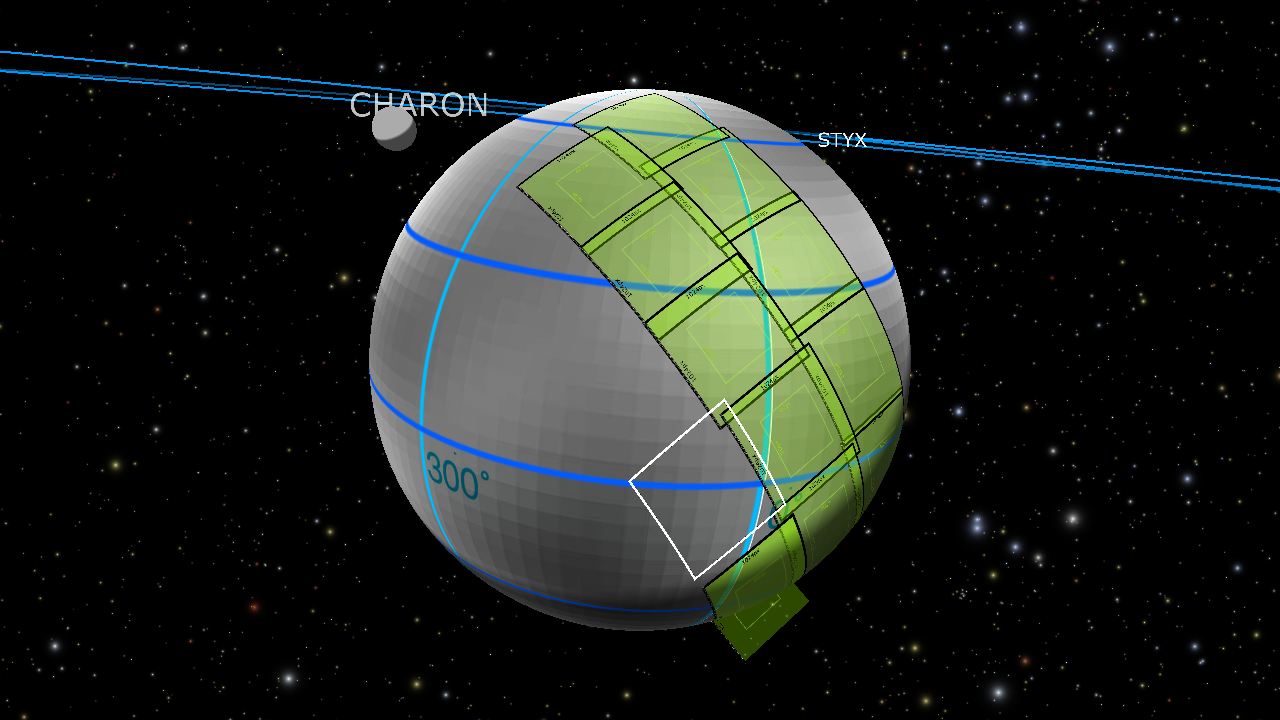
\includegraphics[width=\abOverviewWidth]{figures/pluto.png}}
  \label{fig:pluto}
}
\subfigure[Radio experiment on Pluto's atmosphere] {
  \fbox{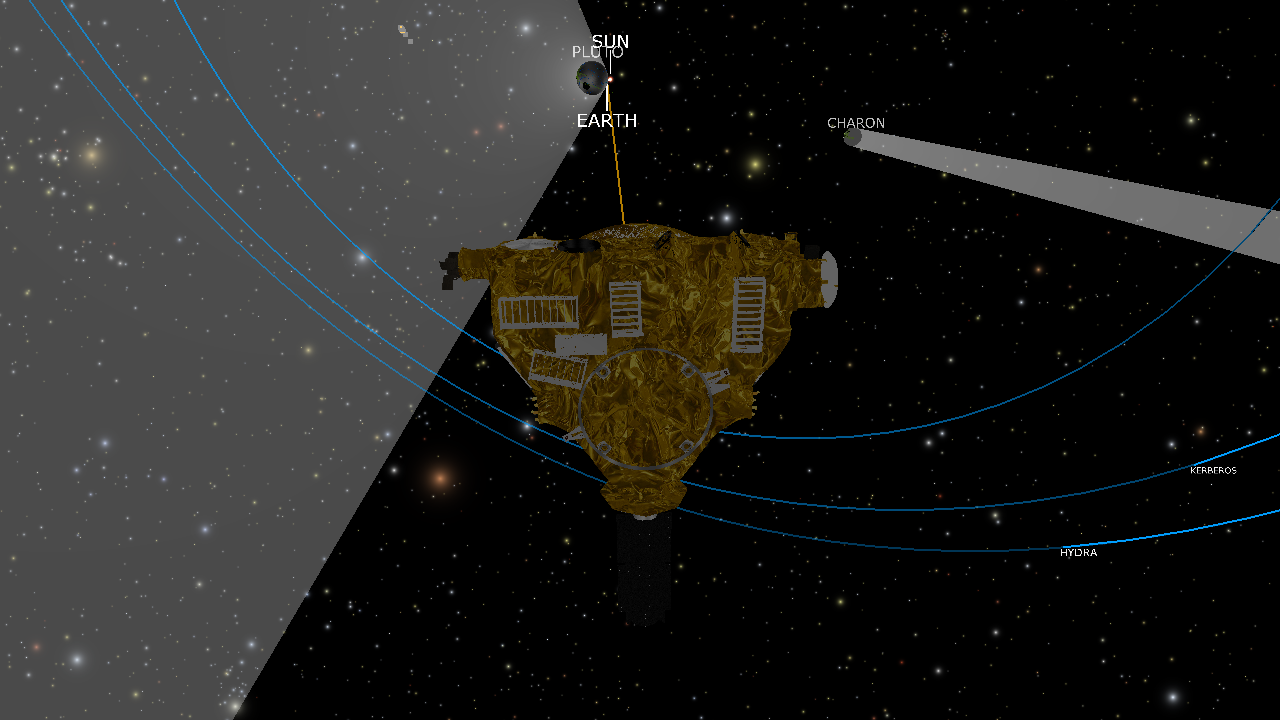
\includegraphics[width=\abOverviewWidth]{figures/pluto2.png}}
  \label{fig:radio}
}
\label{fig:overview}
\caption{Images showing measurements performed by the New Horizons space craft. (a) during a 2007 flyby of Jupiter the space craft imaged the planet for a mosaic image. (b) the projected flyby of Pluto on July 14th, 2015 showing one of the image sequences. (c) the planned REX measurement analyzing the composition of Pluto's atmosphere by receiving a radio signal from earth.}
\end{figure*}


Space missions, such as \emph{New Horizons} or \emph{Cassini}, are very expensive endeavors carried out in the public interest. These missions are planned years in advance in order to maximize the scientific output they produce. Due to this streamlining and the lack of available tools for the general public, the space craft's actions during the scientific exploration can be difficult to understand and communicate. However, the public at large needs to be informed and educated about these processes in order to acknowledge the usefulness of this expense. In our system, we present visualizations to allow the public insight into the mission profiles of select missions and understand the maneuvers and the scientific experiments that are performed. This not only allows the mission scientists to explain their findings in context, but it also allows them to preview different mission plans, while providing interesting content for the public to support future funding.

In this work, we propose a visualization system to integrate various modalities of measurements from space crafts throughout the solar system and present them in a unified way to a lay user that is based on the experiences gained from the very successful software suite \emph{Uniview}~\cite{Klashed:2010tr}. These measurements can be past events, in which the scientific data is available and presented, or planned events, in which the presented data is a placeholder and used to illustrate what measurements the space craft is going to perform. 

The system can be used in one of two ways. First, a user can explore the available data on their own and investigate and discover aspects about a specific mission. This involves moving through time in different mission phases and gain an understanding about the mission and its scientific exploration. Second, instances of the software can be interconnected and remotely controlled for a guided session. This can be accomplished ad-hoc, as well as for a planned event. For planned events, the mission scientists control the visualization and can explain the mission and its details to a greater audience around the world simultaneously. In order to accommodate this, the system is capable of driving multi-projection systems such as powerwalls, dome theaters or planetariums to create an immersive rendering that is shared by hundreds of people.

Our proposed provides the rendering capabilities to, among others (see Figure~\ref{fig:overview}):
\begin{itemize}
\item show models of space craft and planetary bodies in their accurate locations,
\item visualize the active instruments' fields-of-view,
\item map images taken by the space craft onto the target body
\end{itemize}

\section{System}
Our framework called \emph{OpenSpace} is a collaborative open-source development that is focussed on providing a framework that is useful for large-scale, contextualized, multimodal astrovisualization applications. The public dissemination of space craft missions described in this work is the first system to be created and distributed using OpenSpace. Other systems, such as STK~\cite{stk} or Uniview~\cite{Klashed:2010tr}, are either focussed towards the space craft expert and tailored to generating the mission plans, or not open-source, barring the development efforts for smaller projects.

As the contextualization of scientific discoveries is important for gaining knowledge, the framework provides the capabilities for the integrated rendering of geometric models as well as volumetric data using an order-independent transparency algorithm~\cite{Lindholm:2014fm}. Among the contextual cues that are provided to the user are accurate 3 dimensional positions of stars that use the Digital Universe dataset curated by the American Museum of Natural History~\cite{du}. In addition to increased realism, the stars help the user navigate within the solar system and thus provide a vital component. The locations for objects, such as planetary bodies, space craft, or satellites, are calculated using the widely used software suite SPICE~\cite{naif} or by providing the Keplerian elements describing the motion around a parent body.

One of the main science instruments that is used on space craft are digital cameras that take images. In order to present these images to the audience, they are projected onto the target body using projective texturing as described by Everitt~\emph{et al.}~\cite{Everitt:2001tg}. As images are mostly acquired in quick succession, this leads to a mosaic covering of the target, as was done on by the New Horizons mission on Jupiter in 2007 (see Figure~\ref{fig:jupiter}). In the cases where the whole image does not cover a body, a virtual image plane is added that contains the remainder of the image (see Figure~\ref{fig:pluto}).

\subsection{Missions}
The system was developed with the requirements of several missions in mind. However, many capabilities are similar, which allows the reuse of features, such as for the image projection.

\noindent {\bfseries New Horizons.} NASA's mission will fly by the Pluto system on July 14th, 2015 and will take measurements with its seven instruments. Of special interest are the LORRI and RALPH instruments, that will take images of Pluto's and Charon's surface, as well as REX that will take radio measurements of Pluto's atmosphere (see Figure~\ref{fig:radio}). In our system, the images are projected using the method described above and the REX occultation measurements are represented by a line connecting the space craft and Earth. The measurement times for all instruments are presented to the user, but not all instruments have a direct visual mapping, for example the SWAP instrument measures solar wind density values. The components for this mission were shown at the American Museum of Natural History's Evening for Educators event on May 14th that part of the Pluto Palooza event series. In addition, the July 14th fly-by will be shown at various locations around the globe.

\noindent {\bfseries Rosetta.} ESA's mission is currently orbiting the comet 67P Churyumov-Gerasimenko at an altitude of below 100\,km taking measurements and images from the surface. We are using the freely available images from the navigation camera (Navcam) and projecting the images onto a detailed model of the comet (see Figure~\ref{fig:teaser:67p}). This increases the graphical fidelity of the model and allows users to see the movement of the comet underneath the space craft and understand its rotation.

\noindent {\bfseries MIST.} In collaboration with the KTH Royal Institute of Technology, Sweden, we are developing a camera setup for a 3U cubesat, that is a satellite of dimensions 30\,cm$\times$10\,cm$\times$10\,cm. Currently, we are using the proposed system to optimize the location of the camera within the space craft by simulating the camera output from the projected trajectory onto Earth. In a second step, after the space craft has been launched, we will be using the rendering output from this system as a training set for the image reconstruction technique that will be employed~\cite{MKU15}.

\acknowledgements{
The authors would like to acknowledge the New Horizons mission team for their support of the project and providing the projected mission plans, Anton Arbring for his extensive work on the Rosetta image projection, Mattias Malmer for providing the 67P model to the public, and lastly the development team of OpenSpace. The system was implemented using the open-source framework OpenSpace (http://openspace.itn.liu.se).}
%The authors wish to thank A, B, C. This work was supported in part by
%a grant from XYZ.}
%
\bibliographystyle{abbrv}
\bibliography{bibliography}
\end{document}
